\chapter{Commit}

\section{Cara Commit}
\par cara \textit{commit issues} yaitu :

\begin{enumerate}
\item Langkah pertama dengan membuka file yang diletakkan di LocalDisk C-users-namafolder 

\begin{figure}[!htbp]
    \centering
    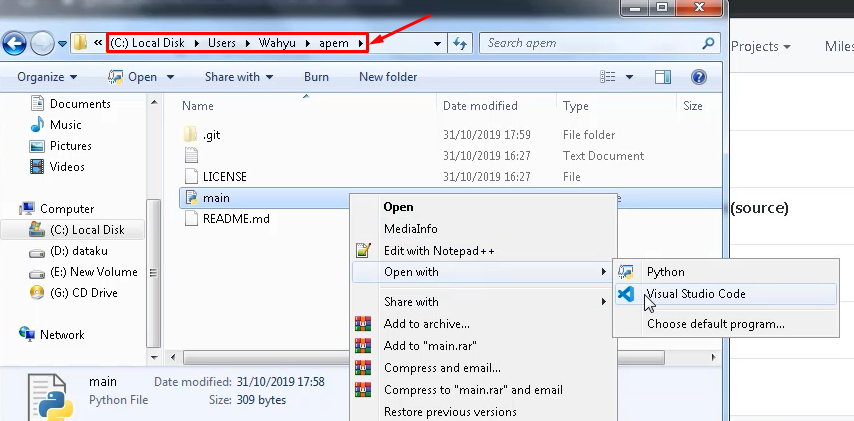
\includegraphics[width=7cm]{figures/file}
    \caption{\textit{file yang akan dicommit}}
\end{figure}

\item kemudian buat tanda "\# issues" untuk menandakan codingan yang terdapat \textit{error}. contoh \textit{error} karena identasi.

\begin{figure}[!htbp]
    \centering
    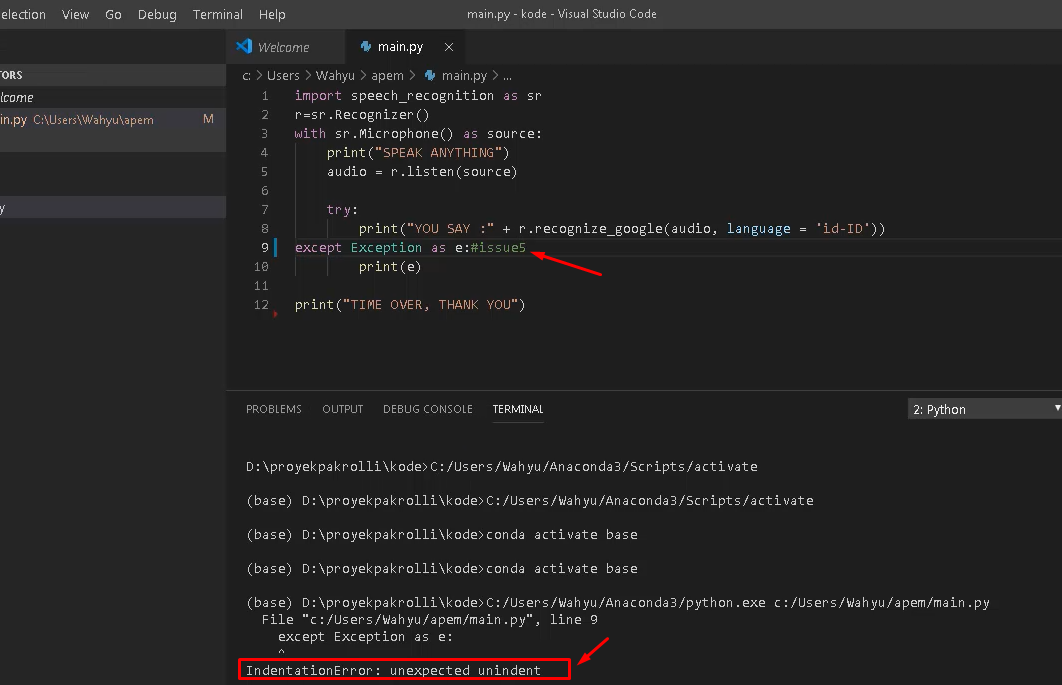
\includegraphics[width=7cm]{figures/error}
    \caption{\textit{error karena identasi}}
\end{figure}

\newpage

\item kemudian buka file yang diletakkan di LocalDiskC-users-namafolder. Kemudian klik kanan pada mouse, kemudian kik \textit{Git Bash here}

\begin{figure}[!htbp]
    \centering
    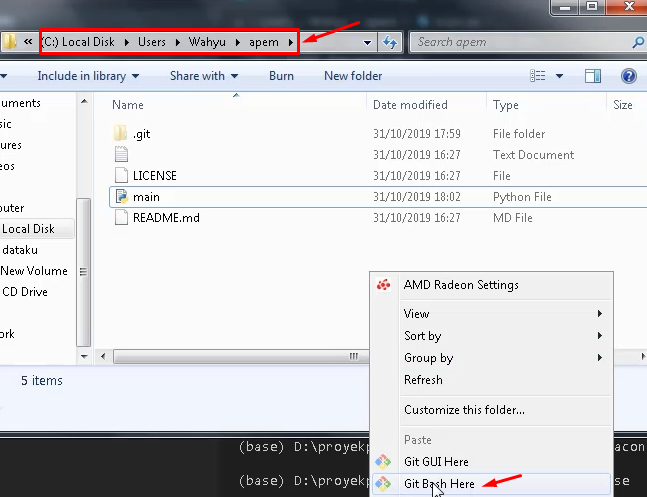
\includegraphics[width=10cm]{figures/bukafolder}
    \caption{\textit{Git Bash here}}
\end{figure}

\item Kemudian ketik

\begin{figure}[!htbp]
    \centering
    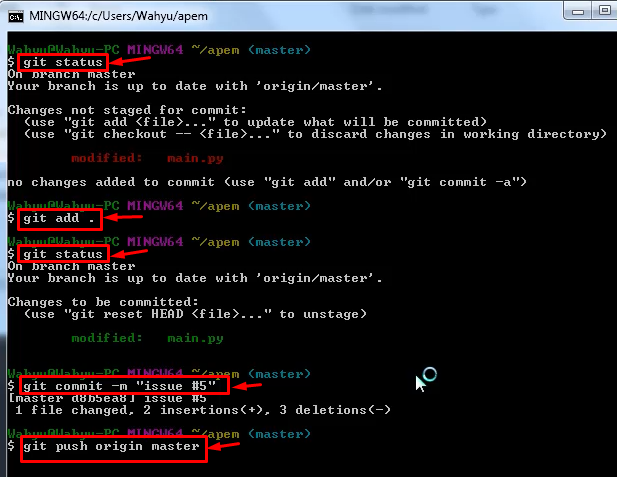
\includegraphics[width=12cm]{figures/git}
    \caption{\textit{cara commit issues}}
\end{figure}

\newpage

\item Kemudian menangani \textit{error} pada codingan, dan beri komentar dengan "\# penyelesaian issues"

\begin{figure}[!htbp]
    \centering
    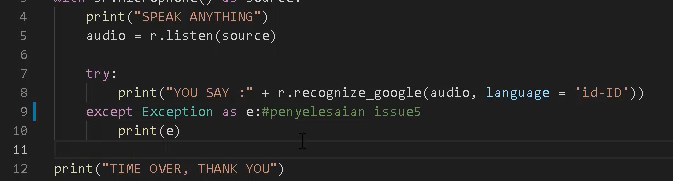
\includegraphics[width=10cm]{figures/atasi}
    \caption{\textit{menangatasi error}}
\end{figure}

\item Buka file yang diletakkan di LocalDiskC-users-namafolder. Kemudian klik kanan pada mouse, kemudian kik \textit{Git Bash here}

\begin{figure}[!htbp]
    \centering
    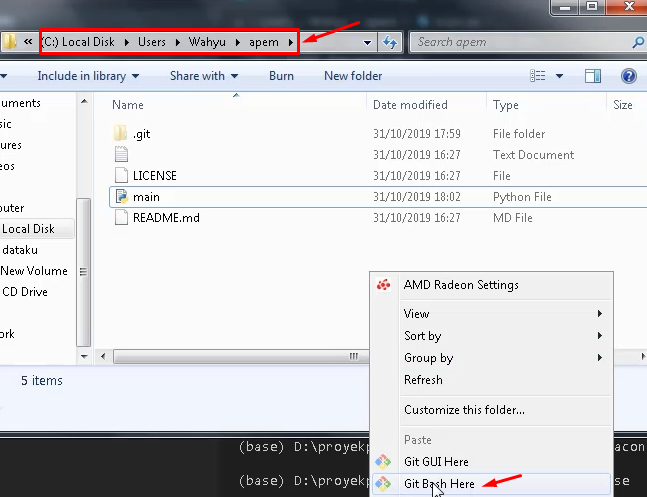
\includegraphics[width=10cm]{figures/bukafolder}
    \caption{\textit{Git Bash here}}
\end{figure}

\newpage

\item kemudian ketik pada cmd

\begin{figure}[!htbp]
    \centering
    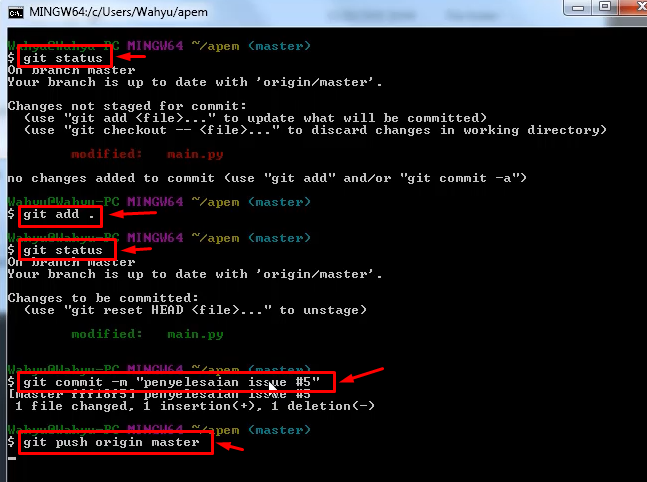
\includegraphics[width=10cm]{figures/ketik}
    \caption{\textit{cara commit issues}}
\end{figure}

\item Buka \textit{issues} yang tadi telah di \textit{commit}, tampilannya seperti ini:

\begin{figure}[!htbp]
    \centering
    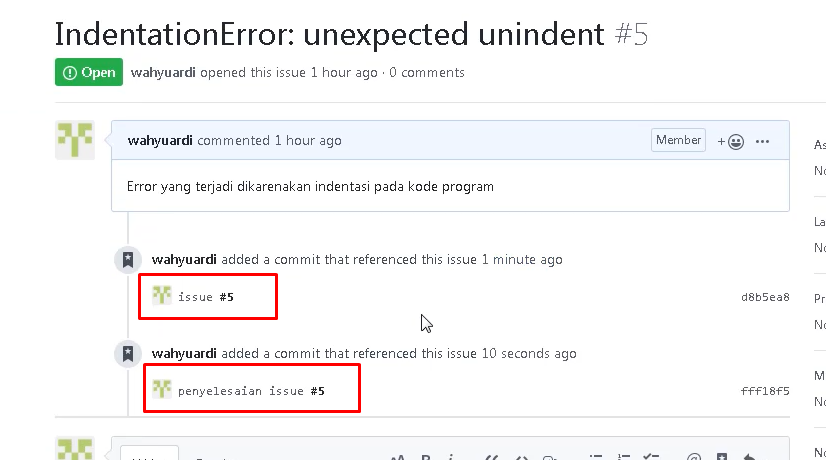
\includegraphics[width=10cm]{figures/errordanpenaganan}
    \caption{\textit{issues error dan issues penyelesaian}}
\end{figure}

\newpage

\item Tampilan \textit{issues error}
\begin{figure}[!htbp]
    \centering
    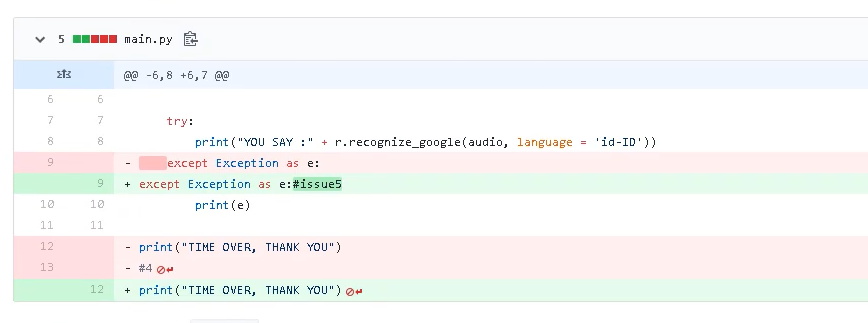
\includegraphics[width=12cm]{figures/tampilanissueserror}
    \caption{\textit{tampilan issues error}}
\end{figure}

\item Tampilan \textit{issues} penyelesaian
\begin{figure}[!htbp]
    \centering
    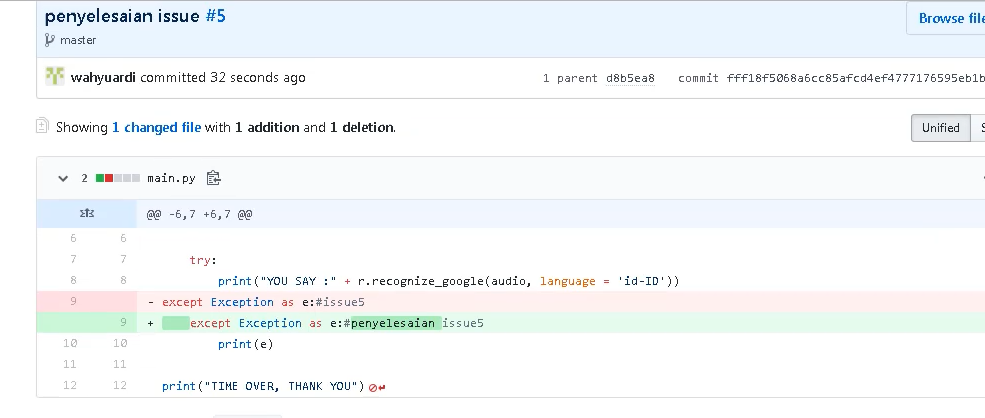
\includegraphics[width=12cm]{figures/tampilanissuespenyelesaian}
    \caption{\textit{tampilan issues penyelesaian}}
\end{figure}

\end{enumerate}

